% COEN 6314 project - two-page data report (v2), single-column article with summary dashboard.
% Compile: pdflatex data_report_v2.tex  (figures are read from fig/)
\documentclass[10pt,a4paper]{article}
\usepackage[a4paper,margin=1.6cm,top=1.4cm,bottom=1.5cm]{geometry}
\usepackage[T1]{fontenc}
\usepackage{lmodern}
\usepackage{microtype}
\usepackage{amsmath}
\usepackage{graphicx}
\usepackage{booktabs}
\usepackage{array}
\usepackage{tabularx}
\usepackage{xcolor}
\usepackage[most]{tcolorbox}
\usepackage{pgfplots}
\pgfplotsset{compat=1.18}
\usetikzlibrary{positioning,arrows.meta}
\usepackage{caption}
\usepackage{titlesec}
\usepackage{enumitem}
\usepackage[hidelinks]{hyperref}

\definecolor{ink}{HTML}{1F2933}
\definecolor{muted}{HTML}{616E7C}
\definecolor{accent}{HTML}{1D5C8C}
\definecolor{tile}{HTML}{EEF3F8}
\definecolor{ctrain}{HTML}{1D5C8C}
\definecolor{cval}{HTML}{E08A2E}
\definecolor{ctest}{HTML}{6B9F59}
\definecolor{ok}{HTML}{3A7D44}

\newcommand{\fn}[1]{\texttt{\detokenize{#1}}}
\newcommand{\done}{\textcolor{ok}{\ding{51}}}
\usepackage{pifont}
\titleformat{\section}{\normalfont\bfseries\color{accent}}{\thesection}{0.5em}{}
\titlespacing*{\section}{0pt}{5pt}{1pt}
\setlength{\parindent}{0pt}
\setlength{\parskip}{2.5pt}
\setlist{nosep,leftmargin=1.1em}
\captionsetup{font=footnotesize,labelfont=bf,skip=2pt}
\newcolumntype{L}{>{\raggedright\arraybackslash}X}
\color{ink}

\newcommand{\kpi}[2]{%
  \begin{tcolorbox}[colback=tile,colframe=tile,arc=2pt,boxrule=0pt,left=1pt,right=1pt,top=2pt,bottom=2pt,
                    width=\linewidth,height=1.15cm,valign=center,halign=center]
  {\large\bfseries\color{accent}#1}\\[1pt]{\scriptsize\color{muted}#2}
  \end{tcolorbox}}

\tikzset{stage/.style={draw=accent!60,fill=tile,rounded corners=2pt,align=center,font=\scriptsize,
                      minimum height=1.05cm,text width=2.5cm,inner sep=2pt},
         arr/.style={-{Stealth[length=4pt]},accent,thick}}

\begin{document}

%================================================================= header
{\LARGE\bfseries PCB Defect Detection Under Image Misalignment}\\[1pt]
{\large Data Report}\hfill{\small Basma Kurany (40374114) \textperiodcentered{} COEN 6314, Concordia University
\textperiodcentered{} November 2026}\\[-5pt]
{\color{accent}\rule{\linewidth}{0.8pt}}

\textbf{Summary.} DeepPCB is a supervised \emph{object-detection} dataset: each defect must be located
(bounding-box \emph{regression}) and labelled with one of six classes (\emph{classification}). We added
\textbf{controlled misalignment}: every validation and test pair is rendered under 10 seeded conditions (as
supplied; 1/2/3/5\,px shifts in $x$ or $y$; a sub-pixel shift with $\leq0.5^\circ$ rotation), boxes moving with the
image, to compare YOLOv10-Nano (trained with and without shift augmentation) against a registration-and-differencing
baseline. \textbf{Statistics} (dashboard): \textbf{1,500} pairs, \textbf{800/200/500} split, \textbf{0--5\,px}
shifts plus a $\leq0.5^\circ$ residual, \textbf{9/9} checks passed.
\textbf{Precautions:} splits are made by board group before augmentation (no board shared by train and val); both
methods read identical shifted files; an 8\,px border is excluded and 258 edge boxes are ignored in every condition.
\textbf{Considerations:} 123 pairs arrive misaligned, 168 test pairs share boards with training and 3 copy train
pairs, so clean and unseen-board subsets are also reported; most defects are synthetic.

\vspace{1pt}\noindent
\begin{minipage}[t]{0.235\linewidth}\kpi{1,500}{image pairs}\end{minipage}\hfill
\begin{minipage}[t]{0.235\linewidth}\kpi{800/200/500}{train / val / test}\end{minipage}\hfill
\begin{minipage}[t]{0.235\linewidth}\kpi{0--5\,px}{misalignment range}\end{minipage}\hfill
\begin{minipage}[t]{0.235\linewidth}\kpi{9/9}{checks passed}\end{minipage}

\vspace{2pt}{\centering
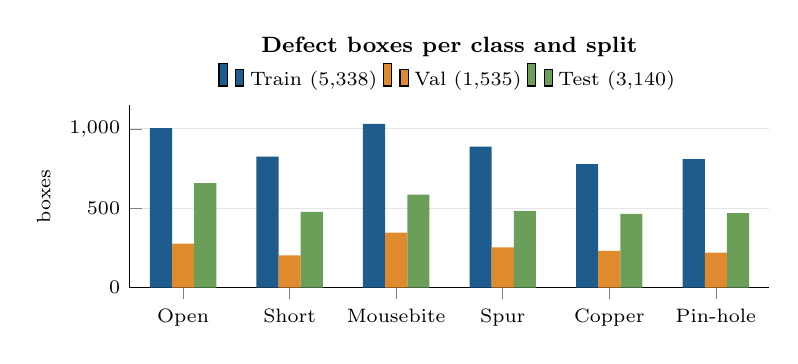
\begin{tikzpicture}
\begin{axis}[
  width=0.8\linewidth, height=3.9cm, ybar=0pt, bar width=8pt,
  symbolic x coords={Open,Short,Mousebite,Spur,Copper,Pin-hole}, xtick=data,
  ymin=0, ymax=1150, ylabel={boxes}, ylabel style={font=\scriptsize},
  tick label style={font=\scriptsize}, axis lines*=left, ymajorgrids, grid style={gray!20},
  legend style={font=\scriptsize, draw=none, fill=none, at={(0.5,1.02)}, anchor=south, legend columns=3},
  title={\footnotesize\bfseries Defect boxes per class and split}, title style={yshift=8pt},
  enlarge x limits=0.1]
\addplot[fill=ctrain,draw=none] coordinates {(Open,1005) (Short,825) (Mousebite,1032) (Spur,888) (Copper,778) (Pin-hole,810)};
\addplot[fill=cval,draw=none]   coordinates {(Open,278) (Short,203) (Mousebite,347) (Spur,254) (Copper,232) (Pin-hole,221)};
\addplot[fill=ctest,draw=none]  coordinates {(Open,659) (Short,478) (Mousebite,586) (Spur,483) (Copper,464) (Pin-hole,470)};
\legend{{Train (5,338)},{Val (1,535)},{Test (3,140)}}
\end{axis}
\end{tikzpicture}\par}

%================================================================= 1
\section{Composition: what the data contains}
DeepPCB~[1] provides 1,500 pairs of $640\times640$ near-binary images, each a defect-free
\emph{template} (reference) and an \emph{inspected} image of the same PCB region, pre-aligned by the authors.
Each pair carries 1--15 boxes (mean 6.7) from six near-balanced classes (largest/smallest ratio 1.33). Defects
are small (median $35\times33$\,px, 0.3\,\% of the image) among many long track edges---the edges misalignment
turns into false differences. The pairs come from 11 board \emph{groups}, the only board identifier.

%================================================================= 2
\section{Preparation pipeline}
All outputs are rebuilt from the untouched download by \fn{scripts/run_all.sh}; seed (6314, pair ID) makes them
reproducible.

\vspace{1pt}{\centering
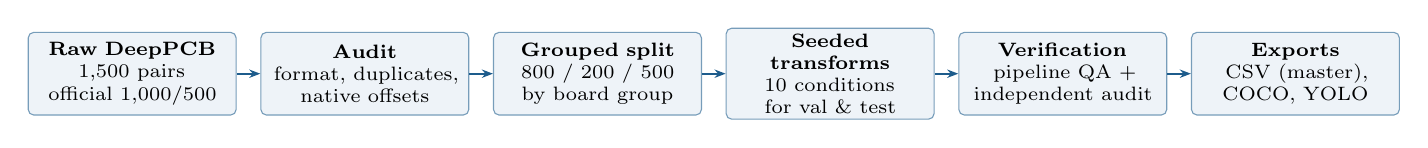
\begin{tikzpicture}[node distance=0.3cm]
\node[stage] (a) {\textbf{Raw DeepPCB}\\1,500 pairs\\official 1,000/500};
\node[stage,right=of a] (b) {\textbf{Audit}\\format, duplicates,\\native offsets};
\node[stage,right=of b] (c) {\textbf{Grouped split}\\800 / 200 / 500\\by board group};
\node[stage,right=of c] (d) {\textbf{Seeded transforms}\\10 conditions\\for val \& test};
\node[stage,right=of d] (e) {\textbf{Verification}\\pipeline QA +\\independent audit};
\node[stage,right=of e] (f) {\textbf{Exports}\\CSV (master),\\COCO, YOLO};
\foreach \x/\y in {a/b,b/c,c/d,d/e,e/f} \draw[arr] (\x) -- (\y);
\end{tikzpicture}\par}

%================================================================= 3
\section{Splits and board leakage}
Crops of the same board look alike, so splitting them across partitions would leak information. DeepPCB has no
board ID; its 11 \emph{group} folders are used as the board unit, and all images of a group are kept together.
\begin{itemize}
\item \textbf{Train vs.\ validation:} about 20\,\% of trainval is held out \emph{before} any augmentation by
assigning whole groups. Among all group subsets holding 17--23\,\% of trainval, group \fn{00041} (200 pairs) has
the class mix closest to trainval ($L_1=0.059$). Train holds the other six groups; the independent audit confirms
no group appears in both. All ten shifted copies of a pair inherit its split.
\item \textbf{Is a group really a board?} Yes: all 40 confirmed near-duplicates lie inside a single group.
\item \textbf{Test:} the official list is kept, but it mixes boards: 168 test pairs come from 7 groups also in
trainval (21 from the validation group) and 3 are near-copies of train pairs. The other 332 come from four groups
never seen in training, so test results are reported on all 500 pairs, on the 332 unseen-board pairs, and without
the 3 duplicates; similar numbers show leakage is not inflating them.
\end{itemize}

%================================================================= 4
\section{Controlled misalignment}
The reference is never modified; the inspected image and its boxes always move together. Each validation and test
pair is given ten conditions, and the baseline and detector read the same files:
\begin{itemize}
\item \fn{s0}: the pair as supplied;
\item \fn{s1x}\dots\fn{s5y}: integer shifts of 1, 2, 3 and 5\,px along $x$ or $y$ (random sign), copied
pixel-exactly with no interpolation;
\item $r$ (residual): a 0.25--1.5\,px sub-pixel translation plus a rotation within $\pm0.5^\circ$ (bilinear), which
whole-pixel registration cannot undo; rotated boxes become the axis-aligned envelope of their corners.
\end{itemize}

\begin{figure}[t]
\centering
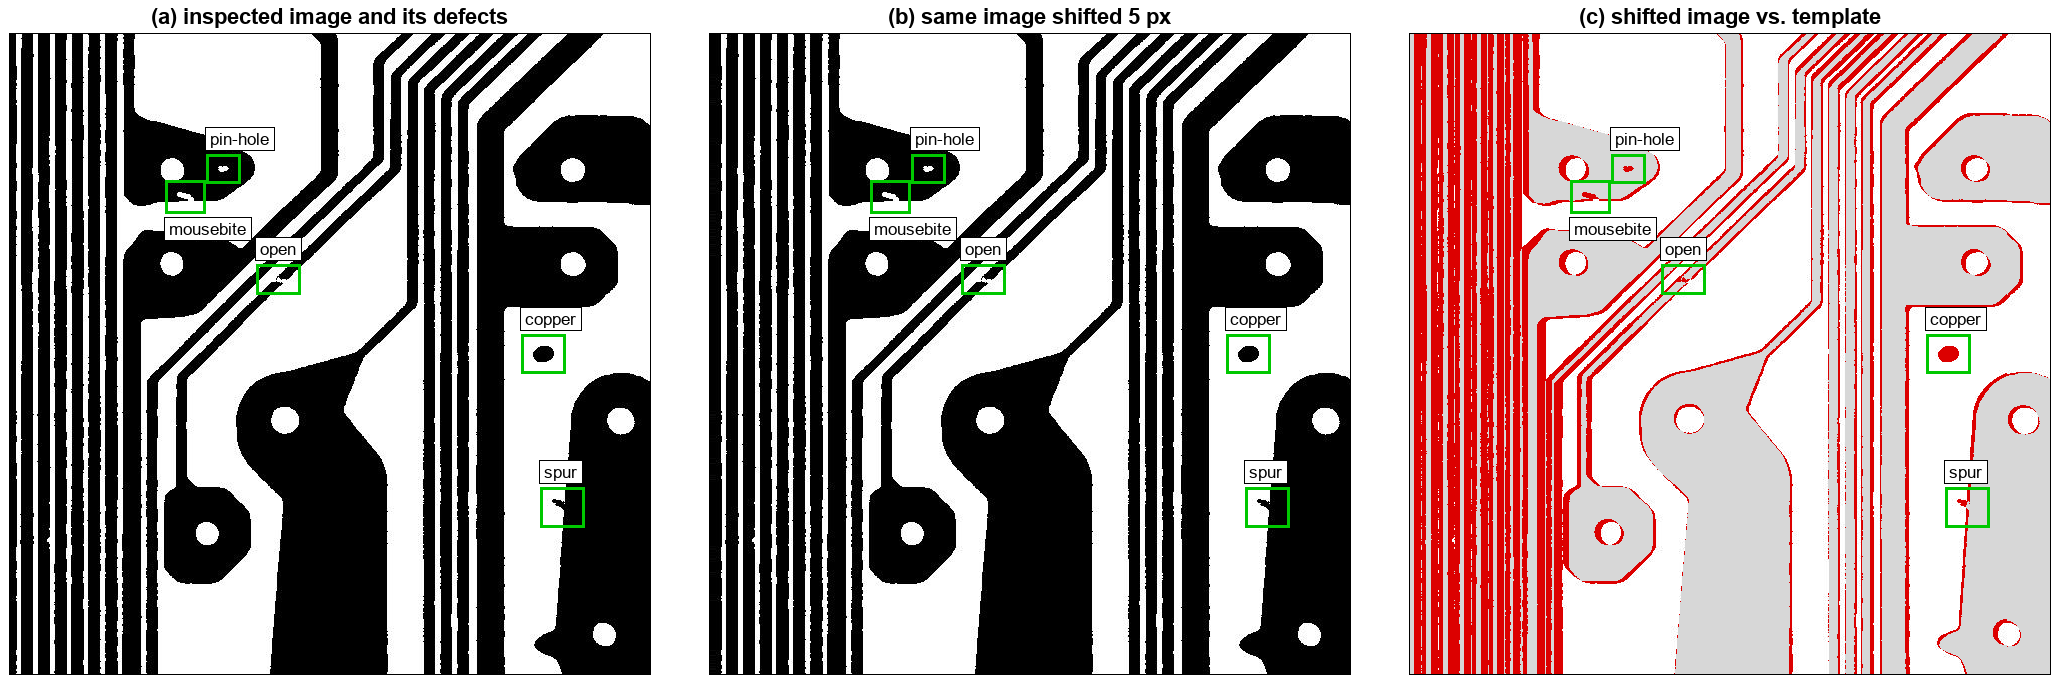
\includegraphics[width=0.68\linewidth]{fig/defect_shift_demo.png}
\caption{Test pair \fn{12300244}: (a) inspected image and its labelled defects; (b) shifted 5\,px with its boxes;
(c) the shifted image vs.\ the unchanged template, red = differing pixels. The shift turns every track edge into a false
difference among the few real defects---what the detector must learn to ignore.}
\label{fig:demo}
\end{figure}
This gives $200\times10=2{,}000$ validation and $500\times10=5{,}000$ test images (46,750 boxes). Outside the
labelled boxes, pixels differing from the template rise from 1.8\,\% of the image as supplied to 6.7\,\% at 5\,px,
i.e.\ from 6 to 16 times the defect pixels. \textbf{Training
does see misalignment:} the non-augmented run uses the 800 pairs as supplied (75 already natively offset), and the
augmented run adds one random 1--5\,px shift and one residual copy of every pair (2,400 images, separate seed
stream; Section~7).
\textbf{Edges:} uncovered pixels lie in an 8\,px border that evaluation excludes; boxes originally within 14\,px of
an edge (258, 2.6\,\%) are \emph{ignored} in every condition: neither hit, miss nor false positive.

%================================================================= 5
\section{Known issues and how they are handled}
\footnotesize
\begin{tabularx}{\linewidth}{@{}>{\raggedright\arraybackslash}p{2.6cm}L>{\raggedright\arraybackslash}p{6.4cm}@{}}
\toprule
Issue & Evidence & Handling\\
\midrule
Native misalignment & 123 ``aligned'' pairs (75/8/40 train/val/test) offset 1--8\,px, mostly 2--3\,px
(XOR area cut $\geq1.5\times$). & Offset stored; also report the 1,377 clean pairs (460 test).\\
Near-duplicates & dHash + pixel check: 40 confirmed, all within one group, none across train/val; 3 test pairs
copy a train pair. & Flagged per pair; report test with and without them.\\
Board overlap & 7 of 11 test groups also occur in trainval (168 pairs). & Unavoidable with the official split;
also report the 332 unseen-board test pairs.\\
\bottomrule
\end{tabularx}
\normalsize

%================================================================= 6
\section{Verification}
\noindent
\begin{minipage}[t]{0.45\linewidth}\vspace{0pt}
Two independent sets of checks were run: the pipeline's QA scripts, and a separate audit that re-decodes the
raw files with a different library (Pillow/SciPy, not OpenCV) and shares no pipeline code. The only difference is
one colour JPEG (\fn{44000020}) whose grey conversion differs between decoders; its shifted copies still match
its own \fn{s0} exactly. Visual sheets like Fig.~\ref{fig:demo} were checked for every condition.
\end{minipage}\hfill
\begin{minipage}[t]{0.52\linewidth}\vspace{0pt}
\footnotesize
\begin{tabular}{@{}p{0.74\linewidth}r@{}}
\toprule
Check & Result\\
\midrule
Pair lists, splits, \fn{boxes.csv} match raw & 1500/1500\\
References identical to raw templates & 1500/1500\\
\fn{s0} identical to raw (independent decoder) & 1499/1500\\
Integer shift $=$ \fn{s0} moved by $(dx,dy)$ & 5600/5600\\
Box count, class, offset, ignore flag & 52088/52088\\
Non-ignored boxes inside valid region & 41220/41220\\
Residual images reproduced from parameters & 700/700\\
COCO files consistent with CSV & 21/21\\
YOLO images with labels, zip CRC intact & 10200/10200\\
\bottomrule
\end{tabular}
\end{minipage}

%================================================================= 7
\section{Intended use and formats}
The master record is a set of CSV files in \fn{index/} (below). They hold annotations and metadata for splitting,
evaluation and error analysis; the detector's input features are the image pixels themselves.

\vspace{2pt}{\centering\footnotesize
\begin{tabularx}{\linewidth}{@{}l>{\raggedright\arraybackslash}p{3.1cm}L@{}}
\toprule
CSV file & One row per & Fields recorded\\
\midrule
\fn{boxes.csv} & original box (10,013) & pair, group, official split, raw corners $x_1,y_1,x_2,y_2$, class, width, height\\
\fn{splits.csv} & source pair (1,500) & pair, group, split, raw paths, box count, native offset + flag, duplicate flag\\
\fn{images.csv} & inspected image (7,800) & image, pair, split, condition, paths, applied $dx$, $dy$, rotation, magnitude, box/ignore counts\\
\fn{labels.csv} & box per image (52,088) & image, pair, split, condition, transformed $x_1,y_1,x_2,y_2$, class (1--6), ignore flag\\
\bottomrule
\end{tabularx}\par}

\vspace{2pt}\textbf{Why COCO:} 21 COCO files (one per split and condition) mirror the CSVs because COCO is the standard
detection format, read by torchvision, Detectron2 and MMDetection (so Fast R-CNN or SSD can be swapped in), and its
\fn{iscrowd} flag makes \fn{pycocotools} treat ignore boxes as don't-care. \textbf{YOLO:} each pair is one 3-channel
image (reference, inspected, $|$difference$|$); the augmented run trains for a third of the epochs (equal steps),
colour augmentation off. Thresholds are set on validation only; test is evaluated once.

%================================================================= 8
\section{Proposal V4 requirements}
\footnotesize
\begin{tabularx}{\linewidth}{@{}L>{\raggedright\arraybackslash}p{8.4cm}c@{}}
\toprule
Requirement (Section 2 of the proposal) & Implementation & \\
\midrule
Official 1,000/500 split; $\sim$20\,\% val before augmentation & 800/200/500; val chosen before any transform & \done\\
Same board and all shifted variants in one partition & Whole groups for train/val; shifted copies inherit split & \done\\
Check cross-partition near-duplicates & 40 confirmed, none train/val; 3 test pairs flagged & \done\\
Reference fixed; image and boxes shifted 0/1/2/3/5\,px in $x$ or $y$ & Conditions \fn{s0}--\fn{s5y}, pixel-exact & \done\\
Residual set: 0.25--1.5\,px and rotation up to 0.5$^\circ$ & Condition $r$, one per val/test pair & \done\\
Identical seeded shifts for both methods & Shared files, seed $(6314,\text{pair ID})$ & \done\\
Exclude padded borders; ignore truncated defects consistently & 8\,px border; 258 boxes ignored in every condition & \done\\
Visually check transformed labels & QA sheets for every condition (Fig.~1) & \done\\
\bottomrule
\end{tabularx}
\normalsize

\vspace{-2pt}\noindent{\footnotesize\textbf{Reference.} [1] S.~Tang \emph{et al.}, ``Online PCB defect detector on a new PCB
defect dataset,'' \emph{arXiv:1902.06197}, 2019.}
\end{document}
